%%%%%%%%%%%%%%%%%%%%%%%%%%%%%%%%%%%%%%%%%%%%%%%%%%%%%%%%%%%%%%%%%%%%%%%%%%%%%%%%%%%%%%%%%%%%%%%%%%%%%%%%%%%%%%%%%%%%%%%%%%%%%%
%%% LaTeX template for the 12º Congresso Iberoamericano de Acústica (12º Congreso Iberoamericano de Acústica) and XXIX Encontro da Sobrac (XXIX Sobrac Meeting)
%%% Based on the Acústica e Vibrações (Sobrac) template
%%% Release 19/04/2022
%%%	Develped by Prof. William D'Andrea Fonseca, Dr. Eng. - Engenharia Acústica UFSM, English revision and translation by Thiago Morphy and Stephan Paul
%%% will.fonseca@eac.ufsm.br
%%%%%%%%%%%%%%%%%%%%%%%%%%%%%%%%%%%%%%%%%%%%%%%%%%%%%%%%%%%%%%%%%%%%%%%%%%%%%%%%%%%%%%%%%%%%%%%%%%%%%%%%%%%%%%%%%%%%%%%%%%%%%%
\documentclass[12pt, a4paper, twoside, twocolumn]{article}
%%%%%%%%%%%%%%%%%%%%%%%%%%%%%%%%%%%%%%%%%%%%%%%%%%%%%%%%%%
%%% Input
\usepackage[utf8]{inputenc} 
\usepackage[english]{babel} % Select the options that fit your needs.
\usepackage[T1]{fontenc}
\usepackage{lmodern, mathptmx} % For Times New Roman
%%%%%%%%%%%%%%%%%%%%%%%%%%%%%%%%%%%%%%%%%%%%%%%%%%%%%%%%%%%%%%%%%%%%%%%%%%%%%%%%%%%%%%%%%%%%%%%%%%%%%%%%%%%%%%%%%%%%
\usepackage{FIA2020} %%% Template basics
%%%%%%%%%%%%%%%%%%%%%%%%%%%%%%%%%%%%%%%%%%%%%%%%%%%%%%%%%%%%%%%%%%%%%%%%%%%%%%%%%%%%%%%%%%%%%%%%%%%%%%%%%%%%%%%%%%%%
%%% Select language options

% For spanish, uncomment the line below
%\Resumen

% For English articles, please do not comment the following line
\SuppressResumo 
%%%%%%%%%%%%%%%%%%%%%%%%%%%%%%%%%%%%%%%%%%%%%%%%%%%%%%%%%%%%%%%%%%%%%%%%%%%%%%%%%%%%%%%%%%%%%%%%%%%%%%%%%%%%%%%%%%%%
%%% Paper data

% \Authors{Fonseca,~W.~D'A.; Last~name,~I.} % For PDF metadata, example for two authors
\Authors{Fonseca,~W.~D'A.} % For PDF metadata

% Use the structure Last name, I
%\AuthorsAffiliations{Fonseca,~W.~D'A.$^1$; Sobrenome,~N.$^2$} % Use numbers to mark the affiliations, example for two authors
\AuthorsAffiliations{Fonseca,~W.~D'A.$^1$} % Use numbers to mark the affiliations

%% Use one line for each author of different affiliations. 
%% If authors share the same affiliation, use the same data and declare different emails.
\Affiliations{$^1$\,Acoustical Engineering Program, Federal University of Santa Maria, Santa Maria, RS, Brazil, will.fonseca@eac.ufsm.br}

% \Affiliations{$^1$\,Acoustical Engineering Program, Federal University of Santa Maria, Santa Maria, RS, Brazil, will.fonseca@eac.ufsm.br\\[2pt]  
% $^2$\,Vibration Laboratory, Institution, City, State, Country, name@domain.com} % Example for two affiliations

\TitleComplete{Instructions and article template for the FIA 2020/22 and\\ XXIX Sobrac meeting}
\TitleShort{Instructions and article template FIA 2020/22 and XXIX Sobrac}              % Short title for the heaing
\TitleEnglish{Instructions and article template for the FIA 2020/22 and XXIX Sobrac meeting} % Additional Title in English for papers written in Portuguese or Spanish

%\PalavrasChave{artigo técnico, FIA, Sobrac, acústica, vibrações} % o Palavras claves
\Keywords{technical paper, FIA, Sobrac, acoustics, vibration}

\PACS{please refer to the instructions in this template}


\Abstract{
This field is intended for the abstract of the article that must contain between 180 and 300 words. Title, abstract, keywords, and PACS should constitute the first page (i.e., avoid extending them to the following page). The abstract should present a concise presentation of the scientific-technical article, containing an introduction, the objective, a synthesis of the method, the main result, and the final conclusion (preferably in that order). No separate items or sections are required within the abstract. Thus, the reader may acknowledge the essence of the article's content. Remember that the abstract is like a \textit{movie trailer}, people will consider reading the complete article if the abstract is interesting. The abstract should not contain new information not contained within the article; undefined abbreviations; previous discussion of the literature; references and citations or excessive detail about the methods employed. It is also not the introductory paragraph of the work; this should be placed at the beginning of the text. Use only relevant and useful information, exercising empathy with prospective readers. For a cohesive and elegant abstract that represents the article, write a preview, write the paper completely, and then review it by looking at whether its content consistently reflects the content of the document. Following the abstract, the author should list up to five keywords (avoid using the same words contained in the article’s title). PACS identifiers, a hierarchical classification system (more details within the text) should be given too.}

\Metadata % Includes the metada into the PDF
%%%%%%%%%%%%%%%%%%%%%%%%%%%%%%%%%%%%%%%%%%%%%%%%%%%%%%%%%%%%%%%%%%%%%%%%%%%%%%%%%%%%%%%%%%%%%%%%%%%%%%%%%%%%%%%%%%%%
%%%%%%%%%%%%%%%%%%%%%%%%%%%%%%%%%%%%%%%%%%%%%%%%%%%%%%%%%%%%%%%%%%%%%%%%%%%%%%%%%%%%%%%%%%%%%%%%%%%%%%%%%%%%%%%%%%%%
\begin{document} \setcounter{page}{1} %%%%%%%%%%%%%%%%%%%%%%%%%%%%%%%%%%%%%%%%%%%%%%%%%%%%%%%%%%%%%%%%%%%%%%%%%%%%%%%%%%%%%%%%%%%%%%%%%%%%%%%%%%%%%%%%%%%%
%%% Template para de LaTeX para o evento 12º Congresso Iberoamericano de Acústica 
%%%                      em conjunto com XXIX Encontro da Sobrac
%%% Baseado no modelo da Revista Acústica e Vibrações da Sobrac
%%% Release 19/04/2022
%%%	Desenvolvido por por Prof. William D'Andrea Fonseca, Dr. Eng. - Engenharia Acústica UFSM
%%% will.fonseca@eac.ufsm.br
%%%%%%%%%%%%%%%%%%%%%%%%%%%%%%%%%%%%%%%%%%%%%%%%%%%%%%%%%%%%%%%%%%%%%%%%%%%%%%%%%%%%%%%%%%%%%%%%%%%%%%%%%%%%%%%%%%%%
%%%%%%%%%%%%%%%%%%%%%%%%%%%%%%%%%%%%%%%%%%%%%%%%%%%%%%%%%%%%%%%%%%%%%%%%%%%%%%%%%%%%%%%%%%%%%%%%%%%%%%%%%%%%%%%%%%%%
%% Estilo do artigo
\pagestyle{plain}
%%%%%%%%%%%%%%%%%%%%%%%%%%%%%%%%%%%%%%%%%%%%%%%%%%%%%%%%%%%%%%%%%%%%%%%%%%%%%%%%%%%%%%%%%%%%%%%%%%%%%%%%%%%%%%%%%%%%
%%% Primeira página
\thispagestyle{firststyle}
% \newgeometry{top=2.1cm, bottom=2cm, left=1.9cm, right=1.9cm, headsep=5mm}
%%%%%%%%%%%%%%%%%%%%%%%%%%%%%%%%%%%%%%%%%%%%%%%%%%%%%%%%%%%%%%%%%%%%%%%%%%%%%%%%%%%%%%%%%%%%%%%%%%%%%%%%%%%%%%%%%%%%
\begin{textblock}{200}(150.2,283.51)
\fontsize{8}{8}\selectfont\sffamily 
DOI:~\href{https://doi.org/\DOIArtigo}{\DOIArtigo}
\end{textblock}
%%% Título
\begin{textblock}{170}(37,12)

\includegraphics[width=0.82\textwidth,page=1]{FIA-logo.pdf}
\end{textblock}

\twocolumn[
\begin{@twocolumnfalse}
\vspace{60pt}
\begin{center}
{\fontsize{18}{22}\selectfont\bfseries 
%% Título
%%%%%%%%%%%%%%%%%%%%%%%%%%%%%%%%%%%%%%%%%%%%%%%%%%%%%%%%%%%%%%%%%%%%%%%%%%%%%%%%%%%%%%%%%%%%%%%%%%%%%%%%%%%%%%%%%%%%
\TituloCompletoArtigo \bookmark[page=1,level=1]{Título e Resumo}
%%%%%%%%%%%%%%%%%%%%%%%%%%%%%%%%%%%%%%%%%%%%%%%%%%%%%%%%%%%%%%%%%%%%%%%%%%%%%%%%%%%%%%%%%%%%%%%%%%%%%%%%%%%%%%%%%%%%
\par}

%%%%%%%%%%%%%%%%%%%%%%%%%%%%%%%%%%%%%%%%%%%%%%%%%%%%%%%%%%%%%%%%%%%%%%%%%%%%%%%%%%%%%%%%%%%%%%%%%%%%%%%%%%%%%%%%%%%
%%%%%%%%%%%%%%%%%%%%%%%%%%%%%%%%%%%%%%%%%%%%%%%%%%%%%%%%%%%%%%%%%%%%%%%%%%%%%%%%%%%%%%%%%%%%%%%%%%%%%%%%%%%%%%%%%%%
\vspace{12pt}
{\fontsize{11}{13}\selectfont \bfseries 
%% Autores
%%%%%%%%%%%%%%%%%%%%%%%%%%%%%%%%%%%%%%%%%%%%%%%%%%%%%%%%%%%%%%%%%%%%%%%%%%%%%%%%%%%%%%%%%%%%%%%%%%%%%%%%%%%%%%%%%%%
\AutoresFiliacoesArtigo
%%%%%%%%%%%%%%%%%%%%%%%%%%%%%%%%%%%%%%%%%%%%%%%%%%%%%%%%%%%%%%%%%%%%%%%%%%%%%%%%%%%%%%%%%%%%%%%%%%%%%%%%%%%%%%%%%%%
\par}

\vspace{2mm}
{\fontsize{9}{11}\selectfont 
%% Filiações
%%%%%%%%%%%%%%%%%%%%%%%%%%%%%%%%%%%%%%%%%%%%%%%%%%%%%%%%%%%%%%%%%%%%%%%%%%%%%%%%%%%%%%%%%%%%%%%%%%%%%%%%%%%%%%%%%%%
\FiliacoesArtigo
%%%%%%%%%%%%%%%%%%%%%%%%%%%%%%%%%%%%%%%%%%%%%%%%%%%%%%%%%%%%%%%%%%%%%%%%%%%%%%%%%%%%%%%%%%%%%%%%%%%%%%%%%%%%%%%%%%%%
\par}
\end{center}

\vspace{-5mm}{\color{FIABlue}\rule{\textwidth}{0.4pt}}
%%%%%%%%%%%%%%%%%%%%%%%%%%%%%%%%%%%%%%%%%%%%%%%%%%%%%%%%%%%%%%%%%%%%%%%%%%%%%%%%%%%%%%%%%%%%%%%%%%%%%%%%%%%%%%%%%%%%
%%%%%%%%%%%%%%%%%%%%%%%%%%%%%%%%%%%%%%%%%%%%%%%%%%%%%%%%%%%%%%%%%%%%%%%%%%%%%%%%%%%%%%%%%%%%%%%%%%%%%%%%%%%%%%%%%%%%
%%% Resumo e palavras-chave
\ResumoTexto
%%%%%%%%%%%%%%%%%%%%%%%%%%%%%%%%%%%%%%%%%%%%%%%%%%%%%%%%%%%%%
%%% Title, abstract and keywords
%%%%%%%%%%%%%%%%%%%%%%%%%%%%%%%%%%%%%%%%%%%%%%%%%%%%%%%%%%%%%
%%% Title
\begin{otherlanguage*}{english}
{\EnglishTitle}
%%%%%%%%%%%%%%%%%%%%%%%%%%%%%%%%%%%%%%%%%%%%%%%%%%%%%%%%%%%%%%%%%%%%%%%%%%%%%%%%%%%%%%%%%%%%%%%%%%%%%%%%%%%%%%%%%%%%
%%%%%%%%%%%%%%%%%%%%%%%%%%%%%%%%%%%%%%%%%%%%%%%%%%%%%%%%%%%%%%%%%%%%%%%%%%%%%%%%%%%%%%%%%%%%%%%%%%%%%%%%%%%%%%%%%%%%
%%% Abstract
		{\textbf{Abstract}} \vspace{5pt}
		
		{\fontsize{11}{12.5}\selectfont
		\AbstractArtigo
		\par}
		%%%%%%%%%%%%%%%%%%%%%%%%% Keywords
		\vspace{0.7\baselineskip} \fontsize{11}{12}\selectfont
		\textbf{Keywords: }{\fontsize{11}{12}\selectfont 
		\KeywordsArtigo.
		\par}
		%%%%%%%%%%%%%%%%%%%%%%%%% PACs:
		\PACSEnglish
	  \vspace{6mm}
\end{otherlanguage*}		
%%%%%%%%%%%%%%%%%%%%%%%%%%%%%%%%%%%%%%%%%%%%%%%%%%%%%%%%%%%%%%%%%%%%%%%%%%%%%%%%%%%%%%%%%%%%%%%%%%%%%%%%%%%%%%%%%%%%
%%%%%%%%%%%%%%%%%%%%%%%%%%%%%%%%%%%%%%%%%%%%%%%%%%%%%%%%%%%%%%%%%%%%%%%%%%%%%%%%%%%%%%%%%%%%%%%%%%%%%%%%%%%%%%%%%%%%
\end{@twocolumnfalse}
]
% \restoregeometry 
% \newgeometry{top=2.1cm, bottom=2cm, left=1.9cm, right=1.9cm, headsep=5mm}
\pagestyle{plain}

%%%%%%%%%%%%%%%%%%%%%%%%%%%%%%%%%%%%%%%%%%%%%%%%%%%%%%%%%%%%%%%%%%%%%%%%%%%%%%%%%%%%%%%%%%%%%%%%%%%%%%%%%%%%%%%%%%%%
% EOF

%%%%%%%%%%%%%%%%%%%%%%%%%%%%%%%%%%%%%%%%%%%%%%%%%%%%%%%%%%%%%%%%%%%%%%%%%%%%%%%%%%%%%%%%%%%%%%%%%%%%%%%%%%%%%%%%%%%%
%%%%%%%%%%%%%%%%%%%%%%%%%%%%%%%%%%%%%%%%%%%%%%%%%%%%%%%%%%%%%%%%%%%%%%%%%%%%%%%%%%%%%%%%%%%%%%%%%%%%%%%%%%%%%%%%%%%%
%%% ARTICLE
%%%%%%%%%%%%%%%%%%%%%%%%%%%%%%%%%%%%%%%%%%%%%%%%%%%%%%%%%%%%%%%%%%%%%%%%%%%%%%%%%%%%%%%%%%%%%%%%%%%%%%%%%%%%%%%%%%%%
%%%%%%%%%%%%%%%%%%%%%%%%%%%%%%%%%%%%%%%%%%%%%%%%%%%%%%%%%%%%%%%%%%%%%%%%%%%%%%%%%%%%%%%%%%%%%%%%%%%%%%%%%%%%%%%%%%%%
\clearpage % It is recommended to leave only the summary data of the first page, however, this is not mandatory.

\section{Introduction}

This template instruction text was developed so that authors can elaborate their articles in a standardized way. The text was adapted from the \href{https://revista.acustica.org.br/acustica/user/setLocale/en_US?source=%2Facustica}{Acoustics \& Vibration Journal} template (originally ``\textit{Acústica e Vibrações}'' from \href{https://www.acustica.org.br/}{Brazilian Society of Acoustics -- Sobrac}), to be used for the 12º Iberoamerican Acoustics Congress integrated with the XXIX Sobrac Meeting. Templates are thought to provide a uniform formatting for all articles of the event. Therefore, in this template, the main guidelines for article elaboration regarding content, graphics, structure, layout presentation, and submission are presented. The template implements the custom styles to format the article properly. The author can, therefore, use this file as a template or model for his article. In addition to the present \LaTeX\xspace (\texttt{.tex}) template, a  Microsoft Word (\texttt{.docx}) template will be available. This version is also available on \href{https://www.overleaf.com/read/hgryywpgmxdx}{Overleaf} and \href{https://github.com/willdfonseca/fia2020}{GitHub}, and is compatible with Windows, Mac, and Linux. Depending on the setup of your TeX distribution, you might be required to download and install additional packages or fonts if you decide to compile locally on your machine. 
Authors are responsible for the article's content, elaboration, and submission in agreement with the present template.

The complete text shall use simple line spacing, using 12-pt Times New Roman font and 0-pt spacing before and 8-pt after paragraphs. The template will take care of this automatically. 
It is common practice to write scientific articles in an impersonal voice; therefore, this practice is recommended. Articles can be written in Portuguese, English, and Spanish\footnote{Foreign language articles written by non-native speakers should, preferably, pass a professional revision.}.

%%%%%%%%%%%%%%%%%%%%%%%%%%%%%%%%%%%%%%%%%%%%%%%%%%%%%%%%%%%%%%%%%%%%%%%%%%%%%%%%%%%%%%%%%%%%%%%%%%%%%%%%%%%%%%%%%%%
%%%%%%%%%%%%%%%%%%%%%%%%%%%%%%%%%%%%%%%%%%%%%%%%%%%%%%%%%%%%%%%%%%%%%%%%%%%%%%%%%%%%%%%%%%%%%%%%%%%%%%%%%%%%%%%%%%%
\section{Basic orientations}

In this section, a summary of how the article should be structured is presented. For more details, check the specific sections of this template.

\vspace{-8pt}
\begin{enumerate} \itemsep=2pt
    \item The provided \LaTeX{} and Word templates contain all configurations required for proper formatting that are described in this document. Moreover, this text simultaneously provides instructions for both writing software.
    \item The first page of an article written in English should feature the title, authors, affiliations, abstract, keywords, and \href{https://pubs.aip.org/DocumentLibrary/files/publications/jasa/Acoustics_PACS.pdf}{PACS}.
    \item The text must be written using the standard language norms.
    \item The maximum number of pages is 12, including the title page and the pages of the appendices, if any.
    \item The size of the paper is A4, with the following margins: 2.0~cm from the top, 2.0~cm from the bottom, 1.8~cm from the left, and also 1.8~cm from the right (spacing between columns is 1.0~cm).
    \item Text must be written in 12-pt Times New Roman, as is in this template.
    \item The article can contain figures, tables, boards, codes, and equations to be placed in the running text. In the text, if necessary, links are allowed to be inserted. Animations are also allowed, as long as they are represented by diagrams in figures. 
    \item A technical article is expected to have a logical, descriptive structure with reproducible content and a list of all references cited in the text.
\end{enumerate}

%%%%%%%%%%%%%%%%%%%%%%%%%%%%%%%%%%%%%%%%%%%%%%%%%%%%%%%%%%%%%%%%%%%%%%%%%%%%%%%%%%%%%%%%%%%%%%%%%%%%%%%%%%%%%%%%%%%
\section{Document and presentation}

Always insert text between sections or subsections, do not orphan them (beginning a section and going directly to the subsection).

%%%%%%%%%%%%%%%%%%%%%%%%%%%%%%%%%%%%%%%%%%%%%%%%%%%%%%%%%%%%%%%%%%%%%%%%%%%%%%%%%%%%%%%%%%%%%%%%%%%%%%%%%%%%%%%%%%%
\subsection{First page}

The first page shall contain the following items to be completed by the authors: title, authors' names, affiliations, abstract, PACS, and keywords. If the complete title is too long, a shorter version is requested to be included in the header of the articles' pages.

The abstract should have between 180 and 300 words. Make sure that the title, authors' names, affiliations, abstract, PACS, and keywords fit on the first page. The abstract should make a concise presentation of the scientific-technical article, containing an introduction, the objective, a synthesis of the methodology, the main result, and the final conclusion (preferably in that order). No separate items or sections are required within the abstract. The reader should be able to capture the essence of the article's content. Remember that the abstract is like a \textit{movie trailer}, people will consider reading the complete article if the abstract is interesting. The abstract should not contain information not contained in the article. Avoid using undefined abbreviations; making discussions of the literature; including references and citations, or excessive detail about the methods employed. It is also not the introductory paragraph of the work; the introduction is to be provided at the beginning of the main text on the next page. Use only relevant and useful information, exercising empathy with prospective readers. For a cohesive and elegant abstract that represents the article, write a preview, write the paper completely, and then review it by looking at whether its content consistently reflects the content of the document.

Following the abstract, the author should list up to five keywords. Avoid using the same words as those in the title of the article.

After that, there is still the 3--5 PACS (Physics and Astronomy Classification Scheme) code presentation, which is a hierarchical classification system created by the American Institute of Physics (AIP). It aids in identifying fields and subfields in physics and related subjects. This classification is used in international journal articles, as well as in some articles to be published in conference proceedings. PACS codes are composed of numbers and letters, e.g., ``43.20.Dk'' for ``Ray acoustic''. 
Authors should search for the best classifications maintained by the AIP at:

\begin{itemize}[noitemsep,topsep=-1ex] \itemsep=8pt
	\item \url{https://asa.scitation.org/pb-assets/files/publications/jas/Acoustics_PACS-1548697226033.pdf}\,.
\end{itemize}
\vspace{0.25em}

PACS codes should be placed after the \textit{resumo} in Portuguese contributions, after the \textit{abstract} in English contributions, and after the \textit{resumen} in Spanish contributions.


For the authors' affiliations, use numbers as superscripts. If there are multiple authors with the same affiliation, use only one address, but add the different e-mails. When the email domain addresses are the same, try to shorten them using braces $\{ \}$. Use a maximum of two lines for each author affiliation. See some of the following examples:
%
\begin{flushleft}
\vspace{-0.5\baselineskip}
\begin{itemize}[topsep=-1ex,align=left,leftmargin=0.2cm] \itemsep=4pt

	\item Fonseca,~W.~D'A.$^1$; Last name,~N.$^2$\\[6pt]	
	$^{1,\,2}$\,Acoustical Engineering Program, Federal University of Santa Maria, Santa Maria, RS, Brazil, 
	 will.fonseca@eac.ufsm.br, name@domain.com.
	
	\item Fonseca,~W.~D'A.$^1$; Mareze,~P.~H.$^2$\\[6pt]	
	$^{1-2}$\,Acoustical Engineering Program, Federal University of Santa Maria, Santa Maria, RS, Brazil,
	\{will.fonseca, paulo.mareze\}@eac.ufsm.br.
	
	\item Fonseca,~W.~D'A.$^1$; Last name,~N.$^2$, Mareze,~P.~H.$^3$\\[6pt]	
	$^{1,\,3,\,2}$\,Acoustical Engineering Program, Federal University of Santa Maria, Santa Maria, RS, Brazil,
	\{will.fonseca, paulo.mareze\}@eac.ufsm.br,\linebreak name@domain.com.

	\item Fonseca,~W.~D'A.$^1$; Last name,~N.$^2$\\[6pt]	
	$^{1}$\,Acoustical Engineering Program, Federal University of Santa Maria, Santa Maria, RS, Brazil,
	will.fonseca@eac.ufsm.br.\\[4pt]		
	$^2$\,Laboratory, Institution, City, State, Country, name@domain.com.	
\end{itemize}
\vspace{-0.4\baselineskip}
\end{flushleft}

%%%%%%%%%%%%%%%%%%%%%%%%%%%%%%%%%%%%%%%%%%%%%%%%%%%%%%%%%%%%%%%%%%%%%%%%%%%%%%%%%%%%%%%%%%%%%%%%%%%%%%%%%%%%%%%%%%%
\subsection{Number of pages}

The complete work should not exceed 12 pages, including the title page, the complete list of references, and appendices, if there are any.

To optimize the space available, figures, tables, and codes must be presented within the body of the text, using one or two columns depending on their content.

%%%%%%%%%%%%%%%%%%%%%%%%%%%%%%%%%%%%%%%%%%%%%%%%%%%%%%%%%%%%%%%%%%%%%%%%%%%%%%%%%%%%%%%%%%%%%%%%%%%%%%%%%%%%%%%%%%%
\subsubsection{Two level subsection examples}

This is a two-level subsection for exemplifying purposes.

%%%%%%%%%%%%%%%%%%%%%%%%%%%%%%%%%%%%%%%%%%%%%%%%%%%%%%%%%%%%%%%%%%%%%%%%%%%%%%%%%%%%%%%%%%%%%%%%%%%%%%%%%%%%%%%%%%%
\subsection{Page and margin sizes}

The size of the page is A4 (210~mm $\times$ 297~mm), and text is to be typeset in two columns, spaced 1.0~cm apart. Headers are different for even and odd pages (as is in this document). Adjust the left and right margins to precisely 1.8~cm, set the bottom margin to 2.0~cm, and the top margin to 2.0~cm. Ensure that you maximize the utilization of all available space. Exceptions can be admitted \eg, when it is required to start a new section, for instance. These can be allocated at the beginning of the next page.

%%%%%%%%%%%%%%%%%%%%%%%%%%%%%%%%%%%%%%%%%%%%%%%%%%%%%%%%%%%%%%%%%%%%%%%%%%%%%%%%%%%%%%%%%%%%%%%%%%%%%%%%%%%%%%%%%%%
\subsection{Characters and Text}

The manuscript should use Times New Roman font, as provided by the template. The title of the article must be placed on the first page, centered, and using 18-pt \textbf{bold} font. Only its first letter is to be capitalized (except for proper names). Spacing after the title is 22-pt. The section titles should use  12-pt \textbf{bold} font, and should be completely capitalized, as presented in this template. Subsection titles use 12-pt \textbf{bold} font, and only their first letter is to be capitalized (unless proper names are included). The running text must use simple spacing, 12-pt font, justified (aligned with both margins of the columns), and no indentation is to be used for the first line of every paragraph. Avoid the use of level three subsections, use a list system instead.

Make use of standard and scientific language in the text\footnote{Footnotes can help in clarifying minor details.}. Foreign words must be written in italics. Initials, acronyms, abbreviations, and/or other compositions that escape from common knowledge should be presented to the reader; e.g., HRTF (\textit{Head-Related Transfer Function}) --- are always written using non-italic font, including in equations. Carry out a grammatical and technical review before submission.

%%%%%%%%%%%%%%%%%%%%%%%%%%%%%%%%%%%%%%%%%%%%%%%%%%%%%%%%%%%%%%%%%%%%%%%%%%%%%%%%%%%%%%%%%%%%%%%%%%%%%%%%%%%%%%%%%%%
\subsection{Spacing between lines and paragraphs}

Simple spacing should be employed between lines, as adopted in this instructive document. The vertical separation between paragraphs is provided by the template. For manual adjustment, Ms~Word users should choose the justified paragraph option (with 8-pt spacing).

%%%%%%%%%%%%%%%%%%%%%%%%%%%%%%%%%%%%%%%%%%%%%%%%%%%%%%%%%%%%%%%%%%%%%%%%%%%%%%%%%%%%%%%%%%%%%%%%%%%%%%%%%%%%%%%%%%%

\begin{figure*}[!ht] %% Example of a two column figure, 
	\centering
	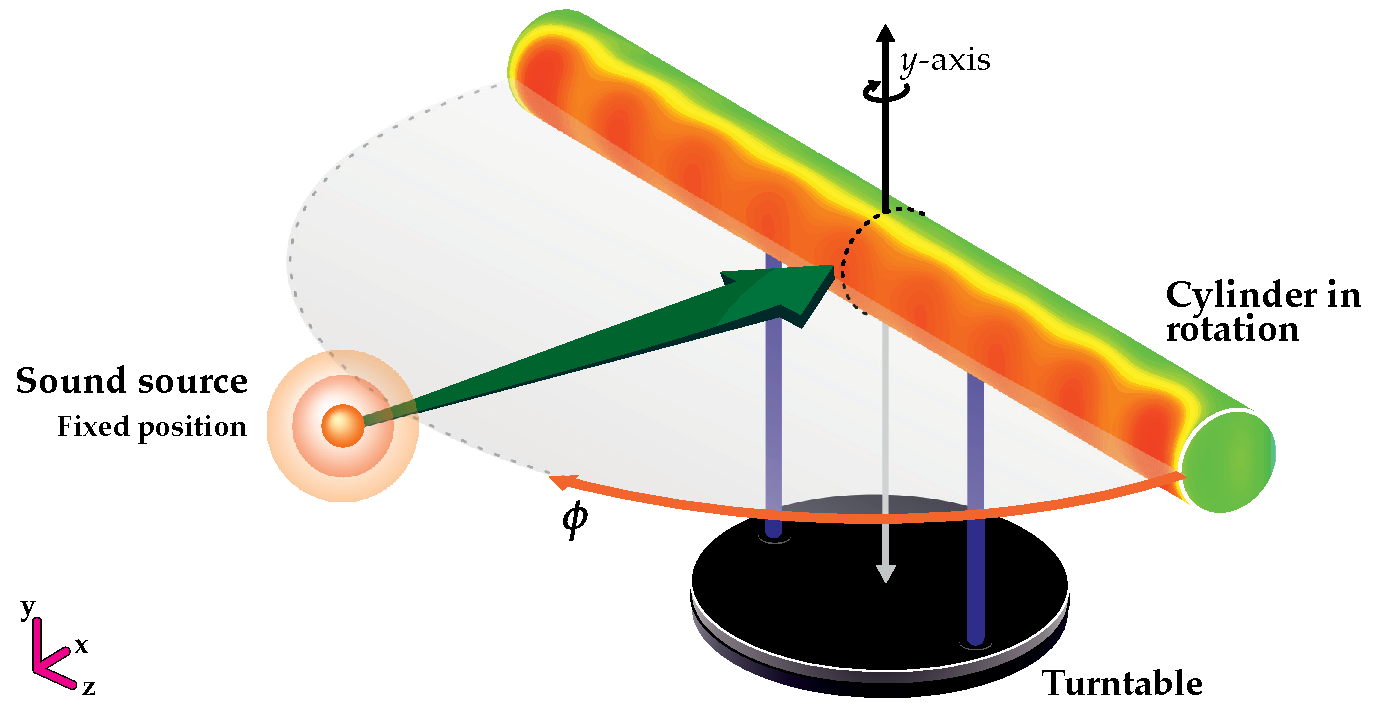
\includegraphics[width=0.74\linewidth]{figs/Measurement-Scheme-Fonseca-2013-en.pdf}%
	\caption{\textit{Beamforming} measurement with cylindrical arrangement (adapted from Fonseca \cite{Fonseca-2013}).\\ Two-columns figure example.}%
	\label{fig:beamforming}%
\end{figure*}

%%%%%%%%%%%%%%%%%%%%%%%%%%%%%%%%%%%%%%%%%%%%%%%%%%%%%%%%%%%%%%%%%%%%%%%%%%%%%%%%%%%%%%%%%%%%%%%%%%%%%%%%%%%%%%%%%%%
\subsection{Equations, variables, and units}

Units of the International System of Units (SI) should be adopted. When writing in Portuguese or Spanish, \textbf{use the comma as decimal separator} in numbers, whether in text, tables, figures, and/or graphics. In addition, make sure to use the same precision when comparing numbers; e.g., 3.0 is different from 3.00 in terms of precision. However, it has the same precision as 6.0. For texts written in English, it is up to the author whether to use a dot or comma as the decimal separator (as long as the notations are not mixed). 

By writing a number and its unit\footnote{Units always use non-italic font, e.g., 30~N/m$^2$.}, always maintain the number along with the corresponding unit, without a line break between them (in Ms~Word, use Ctrl~+~Shift~+~Space [or Alt + 0160], in \LaTeX, insert a tilde ($\sim$) between number and unit). For instance, a distance of 3~m separate the entrance from the exit, or 4.512~cm is the measured distance.

Equations should be inserted in the running text, with proper vertical separations, similar to the example of Equation ~\eqref{fig:beamforming}. Equations should be centralized and enumerated consecutively, this numeration being inserted flush right and between parentheses (see example). Recall that equations are textual elements, therefore, must be properly punctuated and the following text generally does not initiate with an upper-case letter. It is recommended to introduce the nomenclature or definition of a variable immediately after the variable is presented in the equation.

When an already presented equation is to be cited in the text, one should do as follows: Equation~\eqref{eq:densidade} --- with only the first letter in upper case and with the respective number in parentheses.

The circle's area (in m$^2$) is given by
\begin{equation}
	A = \pi \, r^2\;,
\label{eq:area-circ}
\end{equation}
being $r$ the radius in meters (m). 
%
Remember that variables (like $r$ in this example) are written in \textit{italic} (both in equations, text, tables, or figures). When in the running text, no parentheses should be used around the variable because the variable's italic font makes it distinctive from the remainder of the text. 

However, \textbf{units, functions, and mathematical operators} must be written in non-italic font. For instance,``\ldots  32.0~N/m$^2$ was the applied pressure'', or even
%
\begin{equation}
	\int_a^b p(\phi)\, \dt p\,,
\label{eq:int}
\end{equation}
%
was the calculated integral (notice that the differential operator ``d'' is using non-italic font), for each angle $\phi$ in degrees. As mathematical functions, one could mention sine, $\sin(\theta)$, or logarithmic function $\log(y)$, for example.

The subscript or superscript text will only be in italics if corresponding to any pertinent variable. If it is a ``complementary name'' instead, the text shall be written upright, e.g., $P\txu{total}$ corresponds to the total pressure in Pa, or $S\txup{tri}$ corresponds to the triangle area in cm$^2$. However, regarding a variable, for example, $i$ one must write: the summation was calculated considering $P_i$ up to the \textit{i}-th final pressure corresponding to 256. Remember that the imaginary number i is a number, not a variable, and thus should not use italic font, not even in equations.

Text, initials, or units used in equations should also not use italic font, e.g.,
%
\begin{equation}
	\text{density} = \frac{\tx{mass}}{\;\;\tx{volume}\;\;}\,,
\label{eq:densidade}
\end{equation}
%
being the kilogram per cubic meter (kg/m$^3$) the unit of density in the SI system (International System of Units).

%%%%%%%%%%%%%%%%%%%%%%%%%%%%%%%%%%%%%%%%%%%%%%%%%%%%%%%%%%%%%%%%%%%%%%%%%%%%%%%%%%%%%%%%%%%%%%%%%%%%%%%%%%%%%%%%%%%
\subsection{Figures, tables, and codes}

Figures, tables, and codes shall be inserted along the text, by preference following the citing paragraphs that should include a reference to the figures, tables, and codes, respectively. Citation should be made before their actual presentation for the reader's orientation. Interpretation of figures, tables, and codes must be possible without reading the text itself. Figures and tables must be separated vertically from the text by a \textbf{single blank line} (12-pt). The \LaTeX{} template provides this separation automatically.

\begin{table*}[!b]
  \centering \ratb{1.3} 
  \caption{CPA 1 e CAUQ-B porous layers microgeometric and macrogeometric properties \cite{Mareze-2017}.\\ Two-column table example.}
	\fontsize{11}{12}\selectfont 
    \begin{tabular}{C{2.9cm} | C{1.5cm} | C{1.5cm} | C{1.5cm} | C{1.5cm} | C{1.5cm} | C{1.0cm}| C{1.0cm}}
    \toprule
		\SetRowColor{LightOrange}
    \textbf{ Samples / Parameter } & $L\txu{p}$ \qquad [$\upmu$\! m] & $L\txu{a}$ \qquad [$\upmu$\! m] & $D\txu{p}$ \qquad [$\upmu$\! m] & $D\txu{a}$ \qquad [$\upmu$\! m] & $\sigma$ [Ns/m\txup{4}] & {$\phi$\quad [--]} & $\alpha_{\infty}$ [--]\\
	  \midrule
		CPA 1 $\Rightarrow$  3.0\% &	1359.81 & 1492.51 & 2344.05 & 1425.67 &	5131 &	0.218 &	1.63\\
		\rowcolor[gray]{.95} CAUQ-B $\Rightarrow$ 4.5\%	& 1598.29 &	701.24 & 2126.46 & 895.34 &	54989 &	0.070 &	2.89\\
    \bottomrule
    \end{tabular}
    \label{tab.exemplo}%
\end{table*}%

Figures, tables, and codes must be horizontally centralized and sequentially numbered (see examples in Figure~\ref{fig:beamforming}, \ref{subfig.exemplo} and \ref{fig:C80}; Table~\ref{tab.exemplo} and \ref{tab.ex2}; and  Code~\ref{code.matlalatex}). They may be inserted into one or two columns depending on their content. In the case of two columns, it is recommended to position them at the top or bottom of the page. Try to use figures and graphs that present fully comprehensive content. 

The figure's number and label, followed by the title, should appear right below and centralized using 10-pt font. When content produced by other authors is used, even if adapted, indicate the source right after the descriptive title, as seen in the example given in Figure~\ref{fig:beamforming}.

The numbers and titles of the tables and codes must be placed above and centralized (see Table~\ref{tab.exemplo}). The table reference source (when necessary) must be presented in accordance with the original publication. Tables~\ref{tab.exemplo} and \ref{tab.ex2} are presented as examples of the style to be adopted. For the table content, a smaller font (smaller than 12-pt) may be used. Moreover, it is strongly recommended to use the automatic cross reference both in \LaTeX{} as in Ms~Word. Remember that all objects, like figures and tables, must be mentioned in text.

\begin{figure}[H]
\vspace{-0.8em}
  \centering 
	\subfloat[Figure A.]{\label{fig.figA}
\includegraphics[height=23mm,page=2]{FIA-logo.pdf}}
	\qquad
  \subfloat[Figure B.]{\label{fig.figB}
\includegraphics[height=23mm,page=2]{FIA-logo.pdf}}
  \vspace{-0.4em}
  \caption{Side by side figures example.}
  \label{subfig.exemplo}
\end{figure}

\begin{figure}[htb!]
	\centering \vspace{-6mm}
        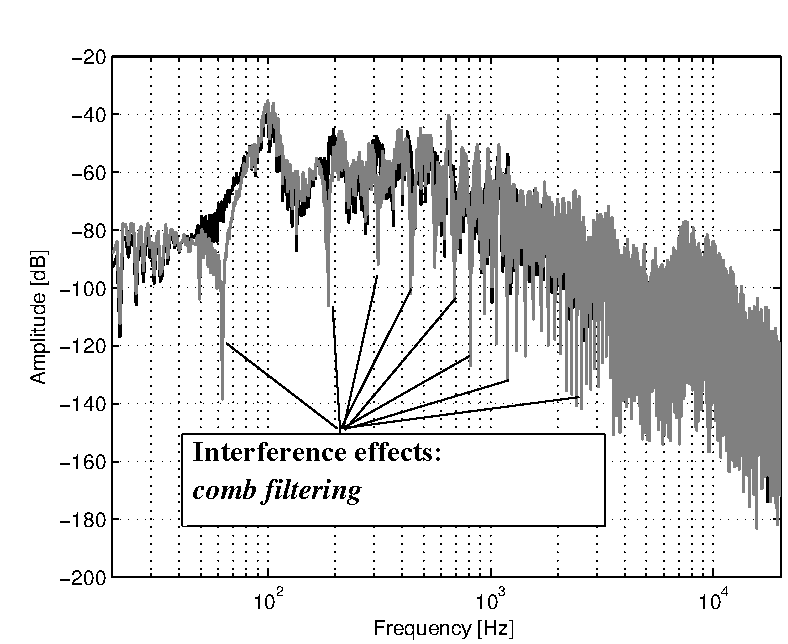
\includegraphics[width=0.98\linewidth,page=1]{figs/Combfilter-Brandao-2017-en.pdf}
        \vspace{-0.5em}
        \caption{$C_{80}$ for distinct rooms. The figures can be inserted side by side (extracted from Brandão \cite{Brandao-2017}).}
	\label{fig:C80}%
\end{figure}

\begin{table}[htb!]
  \centering \ratb{1.3} \setlength\aboverulesep{0pt} \setlength\belowrulesep{0pt}
  \caption{This is an example of a table in one column.}
	\fontsize{11}{12}\selectfont 
    \begin{tabular}{| C{2.8cm} | C{1.8cm} | C{1.8cm} |}
    \hline
	\SetRowColor{LightBlue}
    \textbf{ Experiment / Type } & \textbf{Exp. 1} & \textbf{Exp. 2}\\
	\midrule
		Type~1 & Green & Yellow\\
		\rowcolor[gray]{.95} Type~2 & Blue & White\\
    %\bottomrule
		\hline
    \end{tabular}
    \label{tab.ex2}%
\end{table}%

It is recommended that graphs, figures, and any graph objects are inserted in \!\texttt{.jpg} and/or \texttt{.png} format with good quality (or even in vector form in \texttt{.pdf} for \LaTeX{}\xspace users). Make sure that graphic elements and figures are legible.

The distribution of this \LaTeX\xspace template includes the \texttt{Codes2Latex.sty} package\footnote{The package is still in development and no detailed documentation is available. Hence, for further details, examine the \ttc{sty} file.}, which allows generic code documentation for codes from languages such as Matlab, Fortran, Python, LabView, and \LaTeX{} itself in an organized form (see Code~\ref{code.matlalatex})

\begin{matlabcode}[Making Matlab write Latex.]{code.matlalatex}
  syms x
  f = taylor(log(1+x));
  latex(f)
\end{matlabcode}

All elements (figures and graphs, for example) can be colored or in gray scale. Avoid the use of text elements from other authors without proper citation (and/or authorization). It is essential that text in figures is using the same language as the article. Indirect citations like the ones used in Google Images, for example, will not be accepted, just as it is recommended to avoid the use of volatile knowledge bases.

All figures, tables, and codes must be cross-referenced, for instance: Figure~\ref{fig:beamforming} and Table~\ref{tab.exemplo}. Note that the first letter is capitalized, because both the numbered figure as well as the numbered table is an object with a proper name. Also, the figure's or table's number should not be separated from the word Figure or Table to the next line. To avoid this situation, in Ms~Word, use Ctrl~+~Shift~+~Space, and in \LaTeX, insert a tilde ($\sim$) between the word Figure and the command \verb=\ref= or between the word Table and the command \verb=\ref=.
%
For sub-figures, use Figure~\subref*{fig.figA}, as an example.

%%%%%%%%%%%%%%%%%%%%%%%%%%%%%%%%%%%%%%%%%%%%%%%%%%%%%%%%%%%%%%%%%%%%%%%%%%%%%%%%%%%%%%%%%%%%%%%%%%%%%%%%%%%%%%%%%%%
\section{Article types}

Manuscripts should be \textbf{original submissions} (that is, not yet published) of scientific research and applied engineering, architecture, audio, physics, mathematics, speech and hearing science, and related fields and subfields. Thus, the following document types will be considered:


\begin{itemize}[noitemsep,topsep=-1ex] \itemsep=7pt
	\item \textbf{Technical and applied papers}: present original material based on known and/or developing techniques. Applied methods that are in accordance with regulations and/or present pertinent results must be presented. It is essential that they are of interest to researchers and professionals in the area. 
	
	\item \textbf{Scientific papers}: contain original material (ideas, models, experiments, etc.) not published elsewhere, which substantially contributes to the scientific development. A relationship between the content and the already published \textit{state of the art} must be established.
	
    \item \textbf{Review papers}: discuss the \textit{state-of-the-art} of the intended topic. This type of submission must aim for completeness, covering much of the already developed ideas, models, experiments, etc., even if they are in agreement with the author's opinion. It is important that the subject is of interest of the scientific community.
\end{itemize}

The thematic areas of the event include:
%
\begin{itemize}[noitemsep,topsep=0ex] \itemsep=1.2pt
\item Acoustic materials;
\item Acoustic imaging techniques;
\item Aeroacoustics;
\item Audio and Electroacoustics;
\item Bioacoustics;
\item Building Acoustics;
\item Environmental Acoustics;
\item General Acoustics;
\item INAD and IYS~2020+;
\item Legislation and Standardization;
\item Measurements and Instrumentation in Acoustics and Vibration;
\item Musical Acoustics;
\item Noise and Vibration in the work environment;
\item Noise Control;
\item Numerical methods applied to Acoustics and Vibrations;
\item Psychoacoustics;
\item Room Acoustics;
\item Signal Processing;
\item Soundscapes;
\item Speech and Hearing Acoustics;
\item Teaching in Acoustics;
\item Ultrasound;
\item Underwater Acoustics;
\item Vehicle Acoustics;
\item Vibroacoustics and Vibration; and
\item Virtual Acoustics.
\end{itemize}

%%%%%%%%%%%%%%%%%%%%%%%%%%%%%%%%%%%%%%%%%%%%%%%%%%%%%%%%%%%%%%%%%%%%%%%%%%%%%%%%%%%%%%%%%%%%%%%%%%%%%%%%%%%%%%%%%%%
\section{Arrangement of the sections in the article}

The structure of the article should at least contemplate the following items:
%
\begin{itemize}[noitemsep,topsep=1ex] \itemsep=6pt
    \item Introduction: introduction of the subject, definition of objectives, clarification of relevance;
    \item Fundamentals: especially in scientific articles, the main theoretical foundation required for proper understanding of the reminder of the article must be presented and referenced;
    \item Development: how the work was realized, including theory, materials, and methodological details;
    \item Results and discussions: partial or conclusive, according to the type of work
    \item Conclusion or final considerations: based on the discussion and objectives, arguments or considerations that conclude the study/application must be presented;
    \item Acknowledgments: optional, if pertinent; and
    \item References: list of references that have been cited in the text.
\end{itemize}
%
There is no strict necessity to use the names proposed herein for the sections. The arrangement of the sections can be different depending on the type of article. Other post-textual elements, such as appendices, are optional, as long as the total number of pages of the article, including post-textual elements, does not exceed 12 pages.

%%%%%%%%%%%%%%%%%%%%%%%%%%%%%%%%%%%%%%%%%%%%%%%%%%%%%%%%%%%%%%%%%%%%%%%%%%%%%%%%%%%%%%%%%%%%%%%%%%%%%%%%%%%%%%%%%%%
\subsection{Citations and references}

A separate section named \textbf{References}  must be inserted at the end of the document.

Both in the running text and in the reference list, all references should be \textbf{enumerated according to the order in which they appear in the text}, using brackets \cite{Gomes-2015}. All references listed must be cited in the text. Uncited references should not be added to the list of references. The references given in the template \cite{Mareze-2017,Fonseca-2013,Brandao-2017,Gomes-2015,Oppenheim-1996,Muller-2001,Mareze-2019,Borges-2018,Ristow-2016} are only illustrative.

All entries in the list of references must be formatted in 10-pt Times New Roman font, simple spaced, and 6-pt paragraph spacing. This \LaTeX\xspace template uses the \texttt{natbib} package for the arrangement and formatting of the references. Moreover, the use of bibliography database managers such as \href{http://www.jabref.org/}{JabRef}, \href{http://www.mendeley.com}{Mendeley} and \href{https://www.zotero.org/}{Zotero} is recommended. Especially for Word users, Mendeley has a plugin that formats and can insert references in the \texttt{.docx} document.

Depending on the context, the name of the author may or may not be written when citing in the running text, according to the following examples:

\begin{itemize}[noitemsep,topsep=0ex] \itemsep=4pt
	\item 	``... Mareze \etal \cite{Mareze-2019} worked in porous materials absorption...'', or
	\item ``... for the study of room acoustics~\cite{Brandao-2017}, it is recommended the reading of a textbook...'', or
	\item ``... applying the Fourier transform to the input signals \cite{Oppenheim-1996}. '', or even
	\item ``... Fonseca (2013) demonstrated the diffraction calculation for cylindrical surfaces~\cite{Fonseca-2013}.''
\end{itemize}

All authors appearing in the reference must be cited in text. 
For references with up to three authors, for example,  Müller \& Massarani \cite{Muller-2001}, all authors must be cited (when evoked). In the case of more than three authors, for example, Gomes \etal \cite{Gomes-2015}, only the last name of the first author must be cited, followed by ``\etal''. Still, by citing more than one reference, make use of just one bracket. Some examples are given as follows:

\begin{itemize}[noitemsep,topsep=0ex] \itemsep=8pt
	\item ``Works in Vibration and Acoustics subjects \cite{Mareze-2017,Fonseca-2013,Brandao-2017}.''
	\item ``Works in Acoustics subjects \cite{Mareze-2017,Oppenheim-1996,Muller-2001,Mareze-2019}.''
	\item ``Works with statistical analysis \cite{Mareze-2017, Brandao-2017, Borges-2018}.''
	\item \textbf{Avoid this style:} ``Works with statistical analysis \cite{Mareze-2017}, \cite{Brandao-2017}, \cite{Ristow-2016}.''
\end{itemize}

Compacted and ordered references such as \cite{Mareze-2017,Oppenheim-1996,Muller-2001,Mareze-2019} are recommended.

In the reference section, whenever possible, include ISBN, ISSN, DOI\footnote{For LaTeX users just provide the information in the  ``doi'' field of the  \texttt{.bib} file.} (with link) and/or link to the online address where the cited document is available.

%%%%%%%%%%%%%%%%%%%%%%%%%%%%%%%%%%%%%%%%%%%%%%%%%%%%%%%%%%%%%%%%%%%%%%%%%%%%%%%%%%%%%%%%%%%%%%%%%%%%%%%%%%%%%%%%%%%
\section{Submission and evaluation}

After the submitted abstract has been approved, the authors will be invited to elaborate the complete work. Details about registration and full manuscript submission can be found on the website \url{www.fia2022.com.br}, or can be obtained with the organizing committee.

It is the author's responsibility to submit the articles in their final form, as the organizing committee will not proceed with further adjustments. For this reason, authors are requested to verify the article's formatting with attention, especially graphs and figures, regarding their legitimacy and digital (and print) quality. \textbf{The articles should be sent in PDF format (with a maximum file size of 10~Mb)}.

PDF metadata is automatically generated for \LaTeX\xspace users. Ms~Word users must check during .docx to .pdf conversion.

Studies involving people (or living beings, in general), like in subjective acoustics or physiology, for instance, must inform the ethics committee approval term, if pertinent.

%%%%%%%%%%%%%%%%%%%%%%%%%%%%%%%%%%%%%%%%%%%%%%%%%%%%%%%%%%%%%%%%%%%%%%%%%%%%%%%%%%%%%%%%%%%%%%%%%%%%%%%%%%%%%%%%%%%
\section{Templates for Word and \LaTeX}

The \LaTeX\xspace template (\texttt{.tex}) was written in UTF8 encoding and is thus compatible with Windows, Mac, Linux, and Overleaf. It can be freely used for the article elaboration. We recommend \LaTeX{} users to access the template at \href{https://www.overleaf.com/read/hgryywpgmxdx}{Overleaf}\footnote{\url{https://www.overleaf.com/read/hgryywpgmxdx}.} and create a copy to work on. When downloading the template and working offline with a local \TeX{} distribution, additional packages or fonts might be required and must be downloaded and installed.


The author of the original template and the models is Professor William D'Andrea Fonseca, of the Acoustical Engineering Program (EAC) at the Federal University of Santa Maria (UFSM). 
%
The review was carried out by Professor Stephan Paul (UFSC).
%
The Ms~Word version was created by Felipe Ramos de Mello (EAC/UFSM).

The translation to English was done by Thiago Morphy and Professors Stephan Paul (UFSC) and William D'Andrea Fonseca (UFSM) --- proofreading was carried out by Joseph Lacey.
%
The Spanish version was translated by Diego Martin Tuozzo and revised by William D'Andrea Fonseca and Sicrano.


All templates are available on the \href{http://www.fia2022.com.br}{event website}, \href{https://www.overleaf.com/read/hgryywpgmxdx}{Overleaf} (\href{https://www.overleaf.com/read/rnfjxkknksnd}{PT-BR}, \href{https://www.overleaf.com/read/rszcxtwshzfr}{SP} and \href{https://www.overleaf.com/read/hgryywpgmxdx}{EN}),  and \href{https://github.com/willdfonseca/fia2020}{GitHub}\footnote{\url{https://github.com/willdfonseca/fia2020}.}.

%%%%%%%%%%%%%%%%%%%%%%%%%%%%%%%%%%%%%%%%%%%%%%%%%%%%%%%%%%%%%%%%%%%%%%%%%%%%%%%%%%%%%%%%%%%%%%%%%%%%%%%%%%%%%%%%%%%
\section{Acknowledgments}

If appropriate, acknowledgments should be made. In case of work with financial support, use this section to elucidate details.

In the case of this document, the organization team thanks everyone for their cooperation with the event.

%%%%%%%%%%%%%%%%%%%%%%%%%%%%%%%%%%%%%%%%%%%%%%%%%%%%%%%%%%%%%%%%%%%%%%%%%%%%%%%%%%%%%%%%%%%%%%%%%%%%%%%%%%%%%%%%%%%%
%%%%%%%%%%%%%%%%%%%%%%%%%%%%%%%%%%%%%%%%%%%%%%%%%%%%%%%%%%%%%%%%%%%%%%%%%%%%%%%%%%%%%%%%%%%%%%%%%%%%%%%%%%%%%%%%%%%%
%%% References
\renewcommand{\refname}{References} 
\bibliographystyle{unsrtnat} 
% \bibliographystyle{unsrtnat-br}  % Style similar to Brazilian standards
{\fontrefs \bibliography{bibliografia}}
%%%%%%%%%%%%%%%%%%%%%%%%%%%%%%%%%%%%%%%%%%%%%%%%%%%%%%%%%%%%%%%%%%%%%%%%%%%%%%%%%%%%%%%%%%%%%%%%%%%%%%%%%%%%%%%%%%%
\appendix
\section{Appendix example}

This is an appendix example. Additional information may be included here.

The \LaTeX\xspace template has some additional commands that make writing easier, like, for instance, \F\xspace to symbolize the Fourier Transform. For a better understanding of the commands, consult the \texttt{FIA2020.sty} file.

\end{document}
%%%%%%%%%%%%%%%%%%%%%%%%%%%%%%%%%%%%%%%%%%%%%%%%%%%%%%%%%%%%%%%%%%%%%%%%%%%%%%%%%%%%%%%%%%%%%%%%%%%%%%%%%%%%%%%%%%%
% EOF